\section{Motivation}
Recently, various studies are proposed to exploit the stream feature.
First, Kang et al.~\cite{MultiStream} proposed that the application
is modified to manually assign streams.
Since an application knows the lifetime of the data best, this approach
is very effective in reducing WAF.
However, in order to properly specify streams in the application, the programmer must
fully understand the lifetime characteristics of the data.
Also when multiple applications try to assign streams, a centralized stream assignment
is required to avoid conflicts.
Second, FStream~\cite{FStream} separates short-lived data, e.g., file system metadata and
journal, using the file system information. 
FStream does not require a burden on the programmer, but the system developer is still burdened
to identify short-lived data of the application, e.g., log data of key-value store, based on the file extension.
In addition, those manual techniques are unable to adapt the stream mapping when the workload or application changes.
These limitations of the manual approach can be overcome by the automatic approach.
Lastly, unlike other schemes, AutoStream~\cite{AutoStream} is aimed to automate the process of mapping 
write I/O operations to an SSD stream.
However, since AutoStream relies on the past LBA access patterns, it is not practical when the data are written in
append-only manner, as modern key-value store.

\begin{figure}[!b]
	\vspace{-25pt}
	\centering
	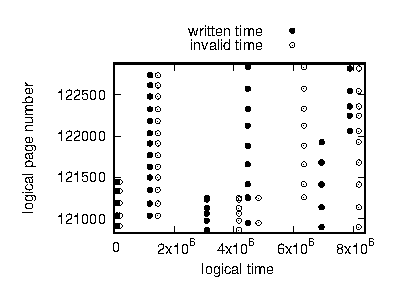
\includegraphics[width=0.9\linewidth]{figure/chunklifetime} % data from 1/02271857 - 59 chunk 
	\vspace{-10pt}
	\caption{The various lifetime of data of append-only workload with in a chunk}
	\label{fig:chunklifetime}
\end{figure}

In order to see how AutoStream work under the append-only workload,
we analyzed the write pattern of RocksDB~\cite{RocksDB}, one of the popular key-value store.
Figure~\ref{fig:chunklifetime} shows the lifetime of the data written to the 1MB-sized logical area.
The x-axis represents the logical time when the data is written and invalidated, and y-axis
represents the logical page number where the data is written to.
As shown in the Figure~\ref{fig:chunklifetime}, the data written to this area had various lifetimes.
It means that the address is not enough to properly distinguish the lifetime of data.
For the automatic stream allocation, thus, more information of the application layer is required.

%The address-based approach can not properly distinguishes the lifetime of the data written by
%the append-only workload.

To sum up, although the application knows the lifetime of the written data, it is hard to 
deliver the information to the system layer without modification.
In this paper, we propose PCStream, which is an automatic stream allocation technique with
more accurate lifetime prediction by obtaining the context informataion of an application.

